\PassOptionsToPackage{table}{xcolor}
\documentclass[10pt]{beamer}
\usepackage[english]{babel}

\usetheme{metropolis}
\usepackage{tikz}
\usepackage{tikz-uml}
\usetikzlibrary{positioning,chains,fit,shapes,calc}
\usepackage{smartdiagram}
\usepackage{listings}
\usepackage{booktabs}
\usepackage[scale=2]{ccicons}%creative commons
\setbeamercovered{transparent}%invisible by default
\usepackage{array}
\newcolumntype{L}[1]{>{\raggedright\let\newline\\\arraybackslash\hspace{0pt}}m{#1}}
\newcolumntype{C}[1]{>{\centering\let\newline\\\arraybackslash\hspace{0pt}}m{#1}}
\newcolumntype{R}[1]{>{\raggedleft\let\newline\\\arraybackslash\hspace{0pt}}m{#1}}

\usepackage{pgfplots}
\usepgfplotslibrary{dateplot}

\newcommand{\mycomment}[1]{}
\usepackage{fancyvrb}
% *****************************************************************************
% Matematica 
% *****************************************************************************

%\usepackage{amssymb}
%\usepackage{mathtools}                    % Add support for cramped,
					  
%\usepackage[euler]{flexisym}
%\usepackage{breqn}                        % Breqn
%\makeatletter
%   \def\eqnumsize{\normalfont \Tf@font}      % Add support to Minion Pro
%\makeatother
%\setkeys{breqn}{labelprefix={eq:}}


%\usepackage{asymptote}
%\usepackage[loop, controls]{animate}

\graphicspath{{./}, {./Images/}}

\lstdefinelanguage{Kotlin}{
  keywords={package, as, typealias, this, super, val, var, fun, for, null, true, false, is, in, throw, return, break, continue, object, if, try, else, while, do, when, yield, typeof, yield, typeof, class, interface, enum, object, override, public, private, get, set, import, abstract, },
  keywordstyle=\color{blue}\bfseries,
  ndkeywords={@Deprecated, Int, Integer, Float, Double, String, Runnable, dynamic},
  ndkeywordstyle=\color{red}\bfseries,
  emph={println, return@, forEach,},
  emphstyle={\color{red}},
  identifierstyle=\color{black},
  sensitive=true,
  commentstyle=\color{gray}\ttfamily,
  comment=[l]{//},
  morecomment=[s]{/*}{*/},
  stringstyle=\color{gray}\ttfamily,
  morestring=[b]",
  morestring=[s]{"""*}{*"""},
}

\providecommand{\ie}{i.\,e.}
\providecommand{\Ie}{I.\,e.}
\providecommand{\eg}{e.\,g.}
\providecommand{\Eg}{E.\,g.} 

\metroset{block=fill}
\metroset{titleformat frame=smallcaps}

\title{The categorical ``flavour'' of the \mbox{Reactive Extensions }(aka Rx)}
\subtitle{and how it can help us building better reactive code}

\date{\today}
\author[A. Candolini]{Alessandro Candolini}
%\institute{Department of Physics, University of Trieste}
% \titlegraphic{\hfill\includegraphics[height=1.5cm]{logo/logo}}

\begin{document}

\maketitle

\begin{frame}%{The man behind reactive extensions}
	\begin{figure}
	\centering
		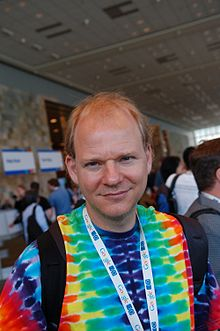
\includegraphics[scale=.5]{ErikMeijer}
		\\
		{Erik Meijer (father of Rx)}
	\end{figure}
\end{frame}

\begin{frame}{Agenda}
  \setbeamertemplate{section in toc}[sections numbered]
  \tableofcontents[hideallsubsections]
\end{frame}

\section{Naive introduction to Rx}
\begin{frame}[fragile]
%\begin{lstlisting}[language=java,basicstyle=\ttfamily,keywordstyle=\color{red}]
\begin{lstlisting}[language=Kotlin, basicstyle=\ttfamily]
/* Observable (data stream) */
val stream: Observable<String> =
            Observable.just("wejd", "adheui", "fe")


/* Observer */
stream.subscribe(
    { s -> println(s) }, /* onNext */
    { t -> println(t) }, /* onError */
    { println("Completed") } /* onComplete */
  )
\end{lstlisting} 
%\frametitle{Warm up}
%\begin{figure}
%		\centering
%		\includegraphics[width=\textwidth]{code1}
%	\end{figure}
\end{frame}
\begin{frame}[fragile]
%\begin{lstlisting}[language=java,basicstyle=\ttfamily,keywordstyle=\color{red}]
\begin{lstlisting}[language=Kotlin, basicstyle=\ttfamily]
val stream: Observable<String> =
            Observable.just("wejd", "adheui", "fe")

stream.map { s -> s.length } //<--
    .filter { l -> l > 2 } //<--
    .subscribe(
       { l -> println(l) },
       { t -> println(t.localizedMessage) },
       { println("Completed") }
    )
\end{lstlisting} 
%\frametitle{Warm up}
%\begin{figure}
%		\centering
%		\includegraphics[width=\textwidth]{code1}
%	\end{figure}
\end{frame}
\begin{frame}[fragile]
%\begin{lstlisting}[language=java,basicstyle=\ttfamily,keywordstyle=\color{red}]
\begin{lstlisting}[language=Kotlin, basicstyle=\ttfamily]
val stream: Observable<String> =
            Observable.just("wejd", "adheui", "fe")

stream.map { s -> s.length }
    .filter { l -> l > 2 }
    .subscribeOn(Schedulers.io()) //<--
    .observeOn(AndroidSchedulers.mainThread()) //<--
    .subscribe(
       { l -> println(l) },
       { t -> println(t.localizedMessage) },
       { println("Completed") }
    )
\end{lstlisting} 
\end{frame}
\begin{frame}[fragile]
%\begin{lstlisting}[language=java,basicstyle=\ttfamily,keywordstyle=\color{red}]
\begin{lstlisting}[language=Kotlin, basicstyle=\ttfamily]
val stream: Observable<String> =
            Observable.just("wejd", "adheui", "fe")

val integers = stream.map { s -> s.length }
      .filter { l -> l > 2 }

integers.subscribeOn(Schedulers.io())
        .observeOn(AndroidSchedulers.mainThread())
        .subscribe(
           { l -> println(l) },
           { t -> println(t.localizedMessage) },
           { println("Completed") }
         )
\end{lstlisting} 
\end{frame}
\begin{frame}[fragile]
%\begin{lstlisting}[language=java,basicstyle=\ttfamily,keywordstyle=\color{red}]
\begin{lstlisting}[language=Kotlin, basicstyle=\ttfamily]
/** Data source */
val stream: Observable<String> =
            Observable.just("wejd", "adheui", "fe")

/** Business logic */
val integers = stream.map { s -> s.length }
      .filter { l -> l > 2 }

/** Consumer */
integers.subscribeOn(Schedulers.io())
        .observeOn(AndroidSchedulers.mainThread())
        .subscribe(
           { l -> println(l) },
           { t -> println(t.localizedMessage) },
           { println("Completed") }
         )
\end{lstlisting} 
\end{frame}
\begin{frame}[fragile]
\begin{lstlisting}[language=Kotlin, basicstyle=\ttfamily]
data class User(name : String) 

interface Repository {
    fun fetchUser(): Observable<User> /*Single??*/
}

repository.fetchUser()
     .map { user -> user.name }
     .subscribeOn(Schedulers.io())
     .observeOn(AndroidSchedulers.mainThread())
     .subscribe(
         { name -> /* Show name */ },
         { t -> /* Show error */  },
         { println("Completed") }
     )       
\end{lstlisting}
\end{frame}

\begin{frame}[fragile]
\begin{lstlisting}[language=Kotlin, basicstyle=\ttfamily]
/* Data source */
val user = repository.fetchUser()

/* Business logic */
val name = user.map { user -> user.name }

/* Consumer layer */
names.subscribeOn(Schedulers.io())
     .observeOn(AndroidSchedulers.mainThread())
     .subscribe(
         { name -> /* Show name */ },
         { t -> /* Show error */  },
         { println("Completed") }
     )       
\end{lstlisting}
\end{frame}



\begin{frame}[fragile]
%\frametitle{Preliminaty feedback}
Naively speaking, Rx provides way to:
	\begin{itemize}
		\item create observables backed by either static or dynamic data
			\begin{itemize}
				\item lists, sensors data, network or db queries, etc
			\end{itemize}
		\item manipulate and combine streams 
		\begin{itemize}\item dot-chaining, built-in operators, etc
			\end{itemize}
		\item observe the stream of events 
	\end{itemize}
%\end{frame}
%\begin{frame}[fragile]
		In addition, Rx provides: 
	\begin{itemize}
		\item propagation of errors along the chain
		\item declarative multithreading  
			\begin{itemize}
				\item parametrize concurrency using schedulers
				\item abstract away low-level threading
			\end{itemize}
	\end{itemize}
\end{frame}
\begin{frame}[fragile]
	\begin{alertblock}{Caution}
		\begin{itemize}
			\item It's \emph{not} an \emph{event bus} (more on this coming soon)
	\begin{figure}
		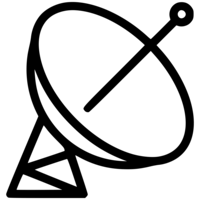
\includegraphics[width=.1\textwidth]{broadcast3}
		\hspace{5ex}
		
\includegraphics[width=.15\textwidth]{broadcast2}
	\end{figure}
			\item It's not a library for (just) abstract away low-level threading
		\end{itemize}
	\end{alertblock}


\end{frame}
\begin{frame}
	%\frametitle{Key ingredients (under the hood) }

	\begin{itemize}
				\item observables are \emph{push-based} (\ie, reactive)
			\begin{itemize}
		\item exploit \emph{duality} (category theory) to \emph{build} observables from iterables 
			\end{itemize}
		\item monadic behavior of observables 
			\begin{itemize}
				\item focus on ``happy path``, propagate exceptions all the way down to the observer 
			\end{itemize}
				\item Provide abstraction on top of asynchronous vs synchronous behavior 
			\begin{itemize}
		\item Rx is parametrised over \emph{concurrency} (\ie, schedulers), not over time
				\item Inversion of control: we can delegate to the consumer  the choice of the schedulers 
			\end{itemize}
		\item \emph{Not just FP}: it does support 
			\emph{side effects} (doOnSomething, Subjects, etc) 
	\end{itemize}

\end{frame}

\section{Categorical duality}

\begin{frame}[fragile]

	\begin{table}
		\rowcolors{2}{gray!25}{white}
		\centering
		\begin{tabular}{C{4cm}|C{4cm}}
			\toprule
			\textbf{Iterable} & \textbf{Observable}\\
			\midrule
			pull-based & push-based \\ 
			interactive & reactive \\
			consumer is in charge & producers is in charge \\
			consumer is active & consumer is passive \\ 
			blocking & non-blocking \\
			no backpressure & backpressure \\ 
			backed by static or dynamic data & backed by static or dynamic data\\
			\bottomrule
\end{tabular}
	\end{table}

\end{frame}


\begin{frame}[fragile]
\begin{lstlisting}[language=Kotlin, basicstyle=\ttfamily]
interface Iterable<out T> {
  fun iterator(): Iterator<T>
}
\end{lstlisting}
\begin{columns}
\begin{column}{0.7\textwidth}
\begin{lstlisting}[language=Kotlin, basicstyle=\ttfamily]
interface Iterator<out T> {
  fun hasNext(): Boolean 
  fun next(): T //<--NoSuchElement
}
\end{lstlisting}
\end{column}
	\begin{column}{0.3\textwidth}
\begin{tikzpicture}
   \umlactor{Active consumer}
\end{tikzpicture}
	\end{column}
\end{columns}
\end{frame}

\begin{frame}[fragile]
	Let's swap arguments and results (mathematical duality).
\begin{lstlisting}[language=Kotlin, basicstyle=\ttfamily]
interface Iterable_<out T> {
   // setter 
   fun set(iterator_: Iterator_<T>) : Unit 
}

interface Iterator_<in T> {
  fun onHasNext(hasNext : Boolean)
  fun onNext(t: T)
  fun onError(error: Throwable)
}
\end{lstlisting}
\end{frame}

\begin{frame}[fragile]
Code cleanup:
\begin{lstlisting}[language=Kotlin, basicstyle=\ttfamily]
interface ObservableSource<out T> {
   fun subscribe(observer: Observer<T>) : Unit
}
\end{lstlisting}
\begin{columns}
\begin{column}{0.7\textwidth}
\begin{lstlisting}[language=Kotlin, basicstyle=\ttfamily]
interface Observer<in T> {
  fun onNext(t: T)
  fun onError(e: Throwable)
  fun onComplete()
}
\end{lstlisting}
\end{column}
\begin{column}{0.29\textwidth}
\begin{tikzpicture}
	\umlactor{Passive consumer}
\end{tikzpicture}
	\end{column}
\end{columns}

\end{frame}



\begin{frame}[fragile]
	\begin{description}
		\item[Iterables] are pull based: it sits until someone asks for \verb|next()| value, you can \emph{iterate} and pull values
		\item[Observables] are pushed based: they decide when to emit values, they \emph{notify} when a new value is pushed
	\end{description}
	\begin{quotation}
		``Earthquakes, in fact, are a really good example of a push based stream. We're not polling the earth for earthquakes.''
	\end{quotation}
	Erik Meijer
\end{frame}


\begin{frame}[fragile]
	Other implications of duality:
	\begin{itemize} 
		\item I can transport results proven for one system into dual results valid for the other system
		\item Duality can be used to achieve \emph{inversion of control}
	\end{itemize}
\end{frame}


\section{Quick (and mostly incomplete) tour about monads}
\begin{frame}{Mathematical functions}
	\begin{figure}
		\centering
		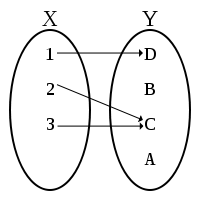
\includegraphics{function}
	\end{figure}
\end{frame}
\begin{frame}
	FP ``keywords'':
	\begin{itemize}
		\item pure functions 
		\item no side effects 
		\item immutability
		\item referential transparency 
	\end{itemize}

	Implications (among other things):
	\begin{itemize}
		\item no loops
		\item no if as a control flow (only as a statement)
		\item no sequence of instructions: just function composition
	\end{itemize}

\end{frame}
\begin{frame}
	Weapons in the FP toolkit:
	\begin{itemize}
		\item Recursion 
		\item Patterns for immutable collections: map, filter, reduce  (we can't use loops)
		\item Algebraic data types \& Pattern matching
		\item Lazyness
		\item And more\ldots 
	\end{itemize}
	But this is not enough. 
\end{frame}
\begin{frame}
Monads can be used 
	\begin{itemize}
		\item as a container 
		\item 
		to structure computations in terms of values and sequences of computations		
	\item to deal with side-effects in a purely functional setting (IO/ asynchronous behaviour, etc) 
 \item  to carry extra data (aka, state) and propagate it through the computation  steps seemlessly 
 \item and many more 
	(the power of a good abstraction)
	\end{itemize}
\end{frame}
\begin{frame}
	\begin{figure}
		\centering
		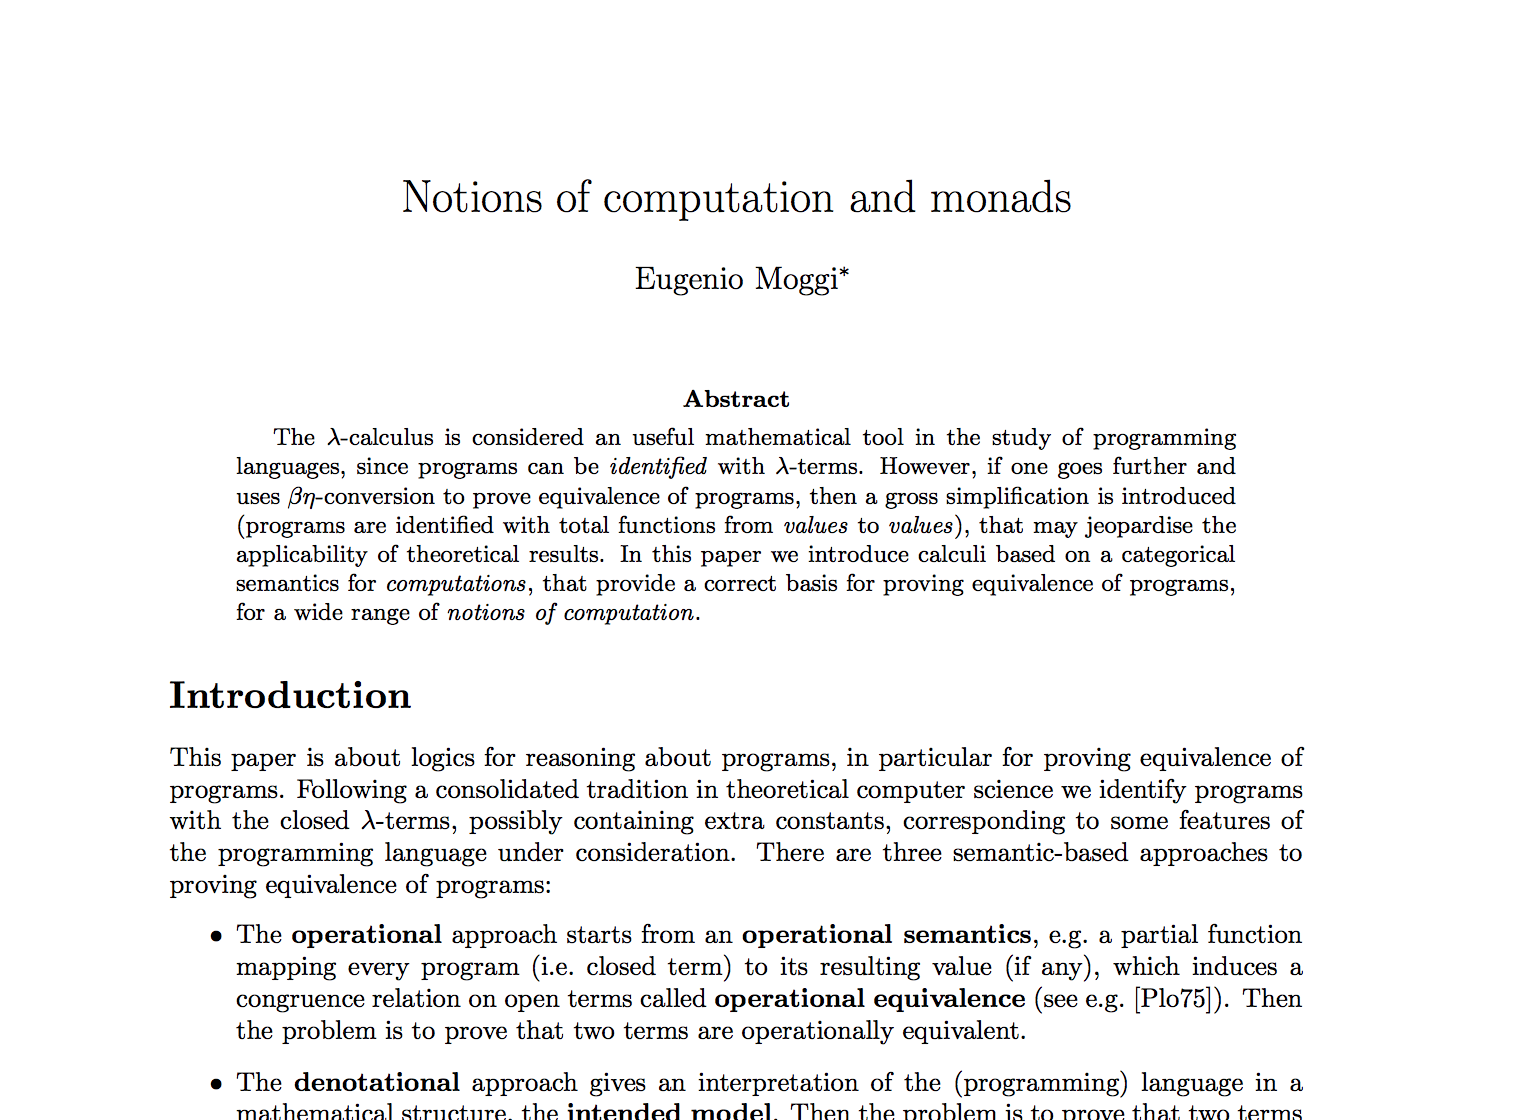
\includegraphics[width=.7\textwidth]{moggi}
		\caption{E. Moggi, Information and Computation
		Volume 93, Issue 1, July 1991, Pages 55-92}
	\end{figure}
\end{frame}
\begin{frame}
	\begin{figure}
		\centering
		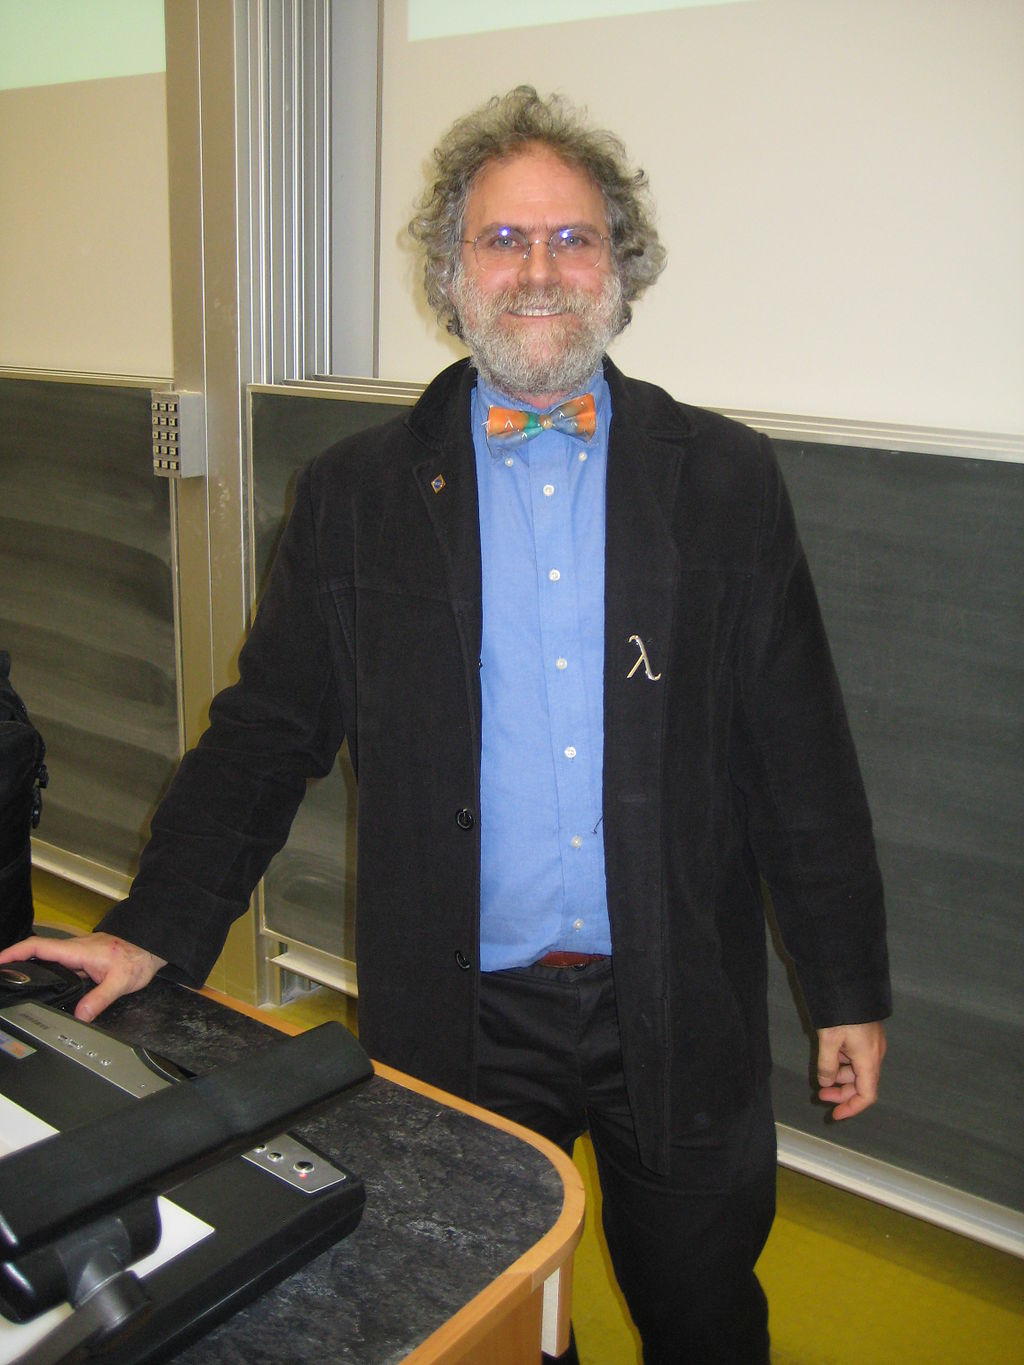
\includegraphics[width=.5\textwidth]{wadler}
		\caption{Philip Wadler (haskell, monads, java generics, and more)}
	\end{figure}
\end{frame}
\begin{frame}\frametitle{What's a monad?}
	\begin{quotation}
		All told, a monad in X is just a monoid in the category of endofunctors of X, with product × replaced by composition of endofunctors and unit set by the identity endofunctor.
	\end{quotation}
	 Saunders Mac Lane in Categories for the Working Mathematician
	\begin{quotation}
		Monads are return types that guide you through the happy path.
	\end{quotation}
	Erik Meijer
	\begin{quotation}
Monads are parametric types with two operations flatMap and unit that obey some algebraic laws.
	\end{quotation}
	Martin Odersky
\end{frame}
\begin{frame}[fragile]
\frametitle{Example (Maybe monad)}
\begin{lstlisting}[language=Kotlin, basicstyle=\ttfamily]
fun f( x : Int ) : Int = x * x
fun g( x : Int, y : Int ) : Int = x/y

val result = f( g( 2,3))
val result = f( g( 2,0)) ??
\end{lstlisting}
Java would naively solve this by using 
	\begin{itemize}
	\item infamous \verb|null|\ldots 
	\item exceptions
	\end{itemize}
\end{frame}
\begin{frame}[fragile]
\frametitle{Example (Maybe monad continuation)}
\begin{lstlisting}[language=Kotlin, basicstyle=\ttfamily]
sealed class Maybe<out T> {
    object None : Maybe<Nothing>()
    data class Just<T>(val t: T) : Maybe<T>()
}
\end{lstlisting}
How to use this?
\begin{lstlisting}[language=Kotlin, basicstyle=\ttfamily]
val j = Maybe.Just(1) 	/* Wrap */
val (i) = j		/* Unwrap */	
\end{lstlisting}
(sealed classes as kind of ADT, \verb|when| as a kind of pattern matching)

In Haskell, more terse syntax\ldots 
\begin{lstlisting}
data Maybe a = Just a | Nothing
\end{lstlisting}
\end{frame}
\begin{frame}[fragile]
\frametitle{Example (Maybe monad continuation)}
\begin{lstlisting}[language=Kotlin, basicstyle=\ttfamily]
fun g( x : Int, y : Int ) : Maybe<Int>
        = if ( y != 0 ) Maybe.Just(x/y)
            else Maybe.None
\end{lstlisting}
Troubles: \emph{composition broken}
\begin{lstlisting}[language=Kotlin, basicstyle=\ttfamily]
val intermediate = g(2,0)
when(intermediate){
  is Maybe.None -> {
      Maybe.None
  }
  is Maybe.Just<Int> -> {
     val (result) = intermediate
     f(result)
  }
}    
\end{lstlisting}
\end{frame}
\begin{frame}[fragile]
	Kleisli triple construction of a monad:
	\begin{description}
		\item[boxing (unit function):] (identity, return, unit): 
			\begin{itemize}
				\item Takes a value from a plain type and puts it into a container using the constructor, creating a monadic value
			\end{itemize}
		\item [unboxing (binding):]  (bind, flatMap):
			\begin{itemize}
				\item 
					The bind operator unwraps the plain value with type a embedded in its input monadic value with type M a, and feeds it to the function.
			\end{itemize}
	\end{description}
			Unboxing allows to ``connect''/``compose''/``link'' sequence of functions  calls by chaining several bind operators together
\end{frame}
\begin{frame}\frametitle{Railway driven development}
	\begin{figure}
		\centering
		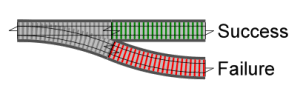
\includegraphics[width=.6\textwidth]{railway1}
	\end{figure}
\end{frame}
\begin{frame}\frametitle{Railway driven development}
	\begin{figure}
		\centering
		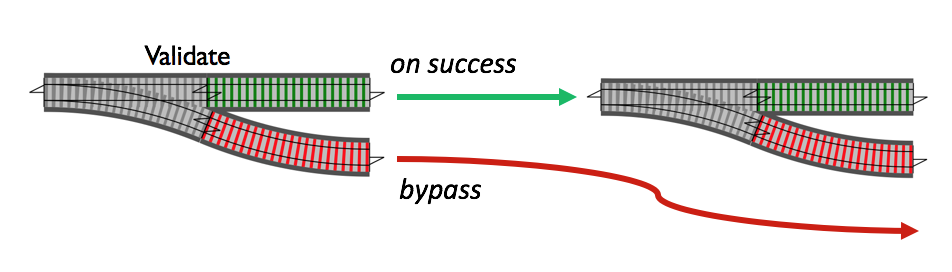
\includegraphics[width=.6\textwidth]{railway2}
	\end{figure}
	Obviously, we cannot compose these two because of the input/output mismatch.
\end{frame}
\begin{frame}\frametitle{Railway driven development}
	\begin{figure}
		\centering
		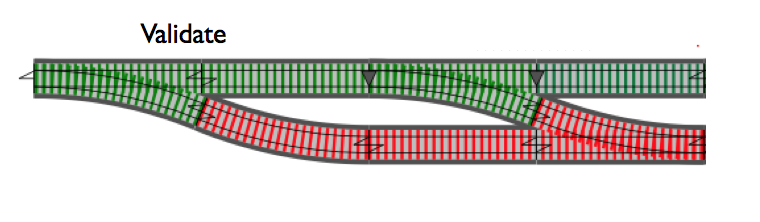
\includegraphics[width=.6\textwidth]{railway3}
	\end{figure}
\end{frame}
%\section{Synch vs asynch behaviour}
\section{Leaving the monad}
\begin{frame}[fragile]
\begin{lstlisting}[language=Kotlin, basicstyle=\ttfamily]
repository.products()
    .doOnNext { products -> println(products) }
    .doOnSubscribe { /* do something*/ }
    .doFinally { /* do something*/ }
    .subscribeOn(Schedulers.io())
    .observeOn(AndroidSchedulers.mainThread())
    .subscribe(
    { products -> /* Show products */ },
    { t -> /* Show error */  },
    { println("Completed") }
    )
\end{lstlisting}
\end{frame}

\begin{frame}[fragile]
\begin{lstlisting}[language=Kotlin, basicstyle=\ttfamily]
class ProductUpdatesManager {

  private val publishSubject
 	= PublishSubject.create<Product>()

  override fun update(product:Product) {
    publishSubject.onNext(product)
  }

  override fun changes() = publishSubject
}
\end{lstlisting}
\end{frame}
\begin{frame}
	\begin{alertblock}
	{Avoid side effects when possible}
	Rx side effects are not different from imperative control flows: they are error prone, inherently difficult to do concurency/asynchronous behaviour, problems with state management, etc (Example: loading spinner) 
	\end{alertblock}
\end{frame}

\begin{frame}
	Subjects are antipatterns:
	\begin{itemize}
		\item Erik Meijer does not like Subjects%
\footnote{\url{https://social.msdn.microsoft.com/Forums/en-US/bbf87eea-6a17-4920-96d7-2131e397a234/why-does-emeijer-not-like-subjects}} :)
		\item  Jake Wharton does not like Subjects either%
\footnote{\url{https://github.com/JakeWharton/RxRelay/issues/7}}
		\item  Subjects $\sim$ non-local side effects%
		\item  Subjects $\sim$ ``global'' state, stateful 
		\item  Subjects implies \emph{fake decoupling}: you think you are decoupling the code (because your subscriber does not now the origin of the values emitted), but actually it means that your \emph{observable source it's not bound}, it can emit everything from everywhere, and this think that you can suddenly receive a new event emitted and you don’t know why, 
		\item Ultimately, subjects $\sim$ event bus / broadcasting, so same drawbacks
	\end{itemize}
\end{frame}

\begin{frame}[fragile]
	Bridge with imperative code can lead to antipatterns
\begin{lstlisting}[language=C++,basicstyle=\ttfamily,keywordstyle=\color{red}]
class WrongPresenter : Presenter {
  fun onButtonClicked() {
     repository.fetch()
               .subscribe(
                 { product -> },
                 { error -> },
                 { }
               )
  }
}
\end{lstlisting}
\end{frame}
\begin{frame}[fragile]
\begin{lstlisting}[language=C++,basicstyle=\ttfamily,keywordstyle=\color{red}]
repository.fetch().subscribe(
    { product -> },
    { error -> when(error) {
          is HttpsURLConnection -> { }
          is SSLException -> { }
          is SQLException -> { }
          else -> { }
        }
    }, { })
\end{lstlisting}
	\begin{quotation}
Anytime you find yourself writing code of the form “if the object is of type T1, then do something, but if it’s of type T2, then do something else,” slap yourself.
	\end{quotation}
	Scott Meyers (Effective C++)
\end{frame}

\plain{Questions?}

%\begin{frame}[allowframebreaks] {References}
% \bibliography{demo}
% \bibliographystyle{abbrv}
%\end{frame}

\end{document}

